\documentclass{article}
\usepackage{pgfplots}
\pgfplotsset{compat=1.18}

\begin{document}

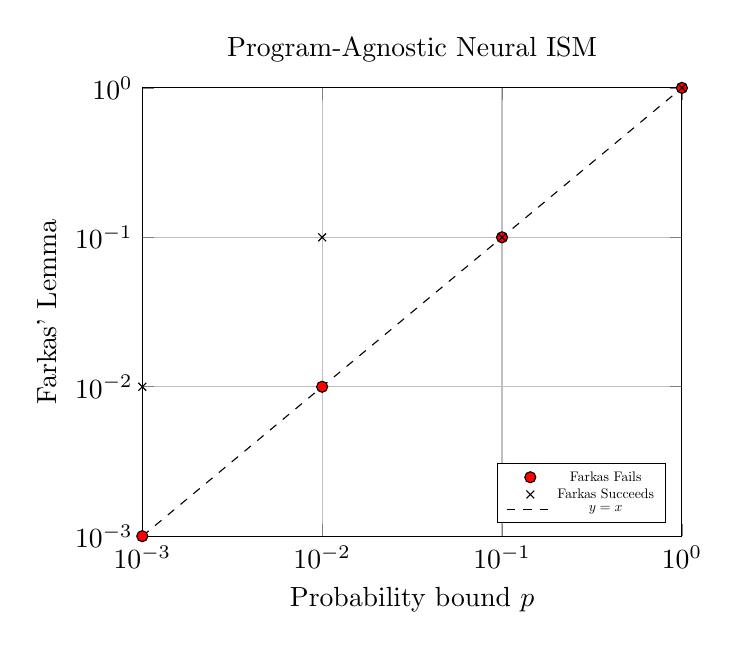
\begin{tikzpicture}
    \begin{loglogaxis}[
        xlabel={Probability bound $p$},
        ylabel={Farkas' Lemma},
        xmin=1e-3, xmax=1,
        ymin=1e-3, ymax=1,
        xtick={1e-3, 1e-2, 1e-1, 1},
        ytick={1e-3, 1e-2, 1e-1, 1},
        legend pos=south east,
        log basis x={10},
        log basis y={10},
        grid=major,
        title={Program-Agnostic Neural ISM},
        legend style={nodes={scale=0.5, transform shape}},
    ]
        % Farkas Fails
        \addplot[only marks, mark options={fill=red}, mark=*] coordinates {
            (1e-3, 1e-3)
            (1e-2, 1e-2)
            (1e-1, 1e-1)
            (1, 1)
        };
        \addlegendentry{Farkas Fails}

        % Farkas Succeeds
        \addplot[only marks, mark options={mark=x, fill=red}, mark=x] coordinates {
            (1e-3, 1e-2)
            (1e-2, 1e-1)
            (1e-1, 1e-1)
            (1, 1)
        };
        \addlegendentry{Farkas Succeeds}

        % Line y = x
        \addplot [dashed, domain=1e-3:1, samples=100] {x};
        \addlegendentry{$y = x$}
    \end{loglogaxis}
\end{tikzpicture}

\end{document}